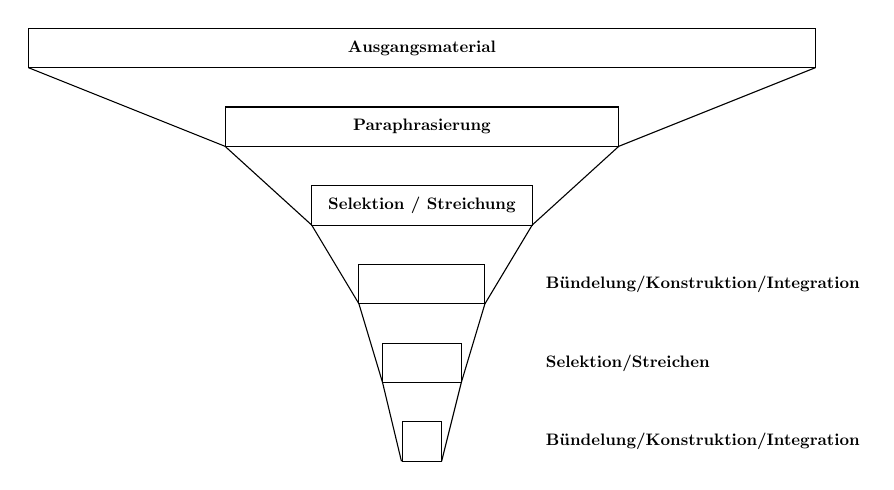
\begin{tikzpicture}

\draw[black, thin] (0,8) rectangle (10,7.5);
\node[draw,scale=0.6,shape=rectangle,draw=none,font=\bf] at (5,7.75) {Ausgangsmaterial};

\draw[black, thin] (2.5,7) rectangle (7.5,6.5);
\node[draw,scale=0.6,shape=rectangle,draw=none,font=\bf] at (5,6.75) {Paraphrasierung};

\draw[black, thin] (3.6,6) rectangle (6.4,5.5);
\node[draw,scale=0.6,shape=rectangle,draw=none,font=\bf] at (5,5.75) {Selektion / Streichung};

\draw[black, thin] (4.2,5) rectangle (5.8,4.5);
\node[draw,scale=0.6,shape=rectangle,anchor=west,draw=none,font=\bf] at (6.5,4.75) {Bündelung/Konstruktion/Integration};

\draw[black, thin] (4.5,4) rectangle (5.5,3.5);
\node[draw,scale=0.6,shape=rectangle,anchor=west,draw=none,font=\bf] at (6.5,3.75) {Selektion/Streichen};

\draw[black, thin] (4.75,3) rectangle (5.25,2.5);
\node[draw,scale=0.6,shape=rectangle,anchor=west,draw=none,font=\bf] at (6.5,2.75) {Bündelung/Konstruktion/Integration};

\draw[black, thin] (0,7.5) -- (2.5,6.5) -- (3.6,5.5) -- (4.2,4.5) -- (4.5,3.5) -- (4.74,2.5);
\draw[black, thin] (10,7.5) -- (7.5,6.5) -- (6.4,5.5) -- (5.8,4.5) -- (5.5,3.5) -- (5.25,2.5);

\end{tikzpicture}